%---------------------------------------------------------------
% Preamble
%---------------------------------------------------------------
\documentclass[a4paper,12pt]{article} 			% Document class
%---------------------------------------------------------------
% Conditionals
%---------------------------------------------------------------
\usepackage{etoolbox}					 		% Toolbox of programming facilities
\usepackage{xpatch}						  		% Extends etoolbox patching commands

%---------------------------------------------------------------
% Paper
%---------------------------------------------------------------
\newtoggle{toclinks}				    	% When editing, add links (next to section titles) to ToC
\newtoggle{cboxes}					   		% When editing, write comments and to-dos
\newtoggle{fulldraft}					 	% Generate short (outline) and long (full draft) versions
\newtoggle{floatstxt}					 	% Put figures and tables in the text or at the end
\newtoggle{blind}					 		% Generate version for journal submission (no identifiers)
\newtoggle{revised}					 		% Highlight changes in revised version
\newtoggle{withappdx}					 	% Include appendix at the end of the paper

\settoggle{toclinks}{true}			   		% 'true' to include ToC and links
\settoggle{cboxes}{true}			   		% 'true' to include boxed comments
\settoggle{fulldraft}{true}	   	 	     	% 'false' to generate an outline
\settoggle{floatstxt}{true}	   	 	 		% 'true' to put figures and tables in the text
\settoggle{blind}{false}	   	 	 		% 'true' to generate version without identifiers
\settoggle{revised}{false}	   	 	 		% 'true' to highlight changes with color
\settoggle{withappdx}{true}	   	 	 		% 'true' to include appendix at the end. Caution: May need to compile paper.tex twice (for ToC) and re-run biber (for references) if the value of this toggle changes

%---------------------------------------------------------------
% Slides
%---------------------------------------------------------------
\newtoggle{stops}					   		% Generate version with stepwise uncovering (more slides)

\settoggle{stops}{true} 					% 'false' for version without stops

%---------------------------------------------------------------
% Paper vs Slides
%---------------------------------------------------------------
\newtoggle{longnotes}					   	% Standalone descrptions in floats: Long for paper, short for slides
\newtoggle{coloreq}					   		% Highlight parts of an equation in slides

\settoggle{longnotes}{true} 				% No need to change it: paper.tex uses it as 'true', each float file sets it to 'false'
\settoggle{coloreq}{false} 					% No need to change it: paper.tex uses it as 'false', slides.tex sets it to 'true' when needed		   		  		% Toggles
%% Packages for Paper
% Contents, Formatting, Math, Figures and Tables,
% Special Characters, Hyperlinks, References

%---------------------------------------------------------------
% Contents
%---------------------------------------------------------------
\usepackage[nottoc]{tocbibind} 		 			% nottoc omits ToC from itself
\usepackage{lipsum}						   		% To add dummy text
\usepackage{pdfpages}					 		% To insert (excerpts of) PDF files
\usepackage[page]{appendix}						% options: titletoc, toc, title, page
	\renewcommand{\appendixpagename}{\centering Appendices}
	\renewcommand{\appendixname}{Appendix}
	\renewcommand{\appendixtocname}{Appendix}
\usepackage{endnotes}							% To place footnotes at the end
%	\let\footnote=\endnote						% Turn on or off as needed
%\usepackage{authblk}					 		% Multiple authors in blocks or in footnotes
%\usepackage{textcomp}		  			 		% Handles the copyright symbol
%\usepackage{makeidx} 							% Creates an index at the end, use \index{} and \printindex

%---------------------------------------------------------------
% Formatting
%---------------------------------------------------------------
\usepackage{pdflscape}			  		  		% To rotate page in PDF using \begin{landscape}
\usepackage{enumerate}				    		% To personalize the enumerate style
\usepackage{titlesec}							% To customize section titles
	\titleformat*{\subsection}{\large\bfseries\itshape}

%---------------------------------------------------------------
% Math
%---------------------------------------------------------------
\usepackage{amsmath} 					 		% For multi-line statements
\usepackage{amssymb} 					 		% For math symbols and fonts
\usepackage{dsfont}								% More math fonts (e.g. indicator function)
%\usepackage{amsthm,enumitem}					% For theorems and control over list environments

%---------------------------------------------------------------
% Figures and Tables
%---------------------------------------------------------------
\usepackage{float}							 	% To enable H placement specifier (similar to h!)
\usepackage{standalone}			   				% To compile sub-files as part of main document
\usepackage{afterpage}					 		% To place floats after current page
\usepackage[labelsep=period,labelfont=bf]{caption} % Caption with dot separator, boldfaced
%	\captionsetup[figure]{position=top}			% To change position of caption
%	\captionsetup[table]{name=New Table Name}	% To change table caption prefix

% Figures
\usepackage{graphicx} 					 		% To include figures
\usepackage[outdir=./]{epstopdf}   				% To avoid errors when calling figures
\usepackage{subcaption}	    	  	   			% Multi-panel figure

% Tables (extensions to standard tabular environment)
\usepackage{tabularx}					 		% For paragraph-like columns
\usepackage{booktabs}			  	   			% For \toprule, \midrule, \bottomrule
\usepackage{multirow}			   				% To add entries with multiple rows
\usepackage{bigstrut} 			 	 		 	% To open up tabular spacing
\usepackage{siunitx}				 	  		% To align the decimal points
\usepackage{threeparttable}		 	  			% To include a structured note section
\usepackage{longtable} 			   				% For multi-page tables
%\usepackage{threeparttablex}		 			% Threeparttable functionality for long tables

%---------------------------------------------------------------
% Special Characters
%---------------------------------------------------------------
\usepackage[style=american]{csquotes}  			% For inline and display quotations
\usepackage[utf8]{inputenc}			  		 	% Handles accented characters (same output on all systems)
%\usepackage[T1]{fontenc}		  	  			% Fonts to use for printing characters
%\usepackage{underscore}				   		% Handles "_" in text but hurts filenames/labels with it

%---------------------------------------------------------------
% Hyperlinks
%---------------------------------------------------------------
\usepackage{xcolor}
	\definecolor{c1}{rgb}{0,0,0} 		   		% Black
	\definecolor{c2}{rgb}{0,0,1} 				% Blue
	\definecolor{c3}{rgb}{0,0,0.54} 		  	% Dark blue
\usepackage[colorlinks=true]{hyperref} 	 		% Creates hyperlinks, 'true' gets rid of the boxes
	\hypersetup{
		citecolor={c1}, 						% Citations
	    linkcolor={c2}, 						% Internal links
	    urlcolor={c3} 							% External links/URLs
	}

%---------------------------------------------------------------
% References
%---------------------------------------------------------------
% To process bibliographic data
\usepackage[style=authoryear,maxbibnames=99,maxcitenames=2,uniquelist=false,uniquename=false,dashed=false,backend=biber]{biblatex}
	\addbibresource{../References/library.bib} 		%Imports the bibliography file 

% General
\renewcommand\multicitedelim{\addcomma\space}	% Citations separated by a comma
\uspunctuation									% Activate ‘American-style’ punctuation
%\stdpunctuation								% Restores standard punctuation

% Customize all types
\DeclareDelimFormat[bib]{nametitledelim}{\addspace} % Remove dot after year
\xpretobibmacro{date+extradate}{\setunit{\addperiod\space}}{}{}	% Dot after author
\renewbibmacro{in:}{} 							% No in: before title

% Customize book type
\DeclareFieldFormat[book]{title}{#1}		  	% Non-italic book title

% Customize report type
\DeclareFieldFormat[report]{pages}{#1}			% No pp. before pages
\DeclareFieldFormat[report]{title}{\mkbibquote{#1\isdot}} % % Title in quotations and not in italics

% Customize article type
\DeclareFieldFormat[article]{pages}{#1} 		% No pp. before pages
\AtEveryBibitem{								% Omit fields
	\ifentrytype{article}{
		\clearfield{doi}%
		\clearfield{url}%
		\clearfield{urldate}%
		\clearfield{issn}%
		\clearfield{eprint}%
		\clearfield{review}%
		\clearfield{series}%%
		\clearfield{month}%%
	}{}
}
\renewbibmacro*{volume+number+eid}{%			% Redefine to remove dot after volume
	\printfield{volume}%
	\setunit*{\addnbspace}%
	\printfield{number}%
	\setunit{\addcomma\space}%
	\printfield{eid}}
\DeclareFieldFormat[article]{number}{\mkbibparens{#1}} % Parenthesis around volume number		   		  	% Packages
%% Page Settings
% Margins, Head and Foot, Indentation, Spacing, Hyphenation,
% Date Format, Thanks Symbols, Reset Float Defaults, Footnotes

%---------------------------------------------------------------
% Margins
%---------------------------------------------------------------
\usepackage[margin=1in]{geometry}	 		% Sets the margins of the file
%\usepackage[top=2.54cm,bottom=2.54cm,left=3.17cm,right=3.17cm]{geometry}

%---------------------------------------------------------------
% Head and Foot
%---------------------------------------------------------------
\usepackage{fancyhdr} 						% For head and foot options

%---------------------------------------------------------------
% Indentation
%---------------------------------------------------------------
\parindent=15pt 				 			% 15pt is the default in one-column documents

%---------------------------------------------------------------
% Spacing
%---------------------------------------------------------------
\usepackage{setspace}
	\doublespacing
	%\setlength{\abovedisplayskip}{1pt}  	% Sets spaces above/below an equation
	%\setlength{\belowdisplayskip}{1pt}
\AtBeginDocument{							% Avoids excesive spacing b/w floating objects
	\addtolength\abovedisplayskip{-0.2\baselineskip}
	\addtolength\belowdisplayskip{-0.2\baselineskip}
}

%---------------------------------------------------------------
% Hyphenation
%---------------------------------------------------------------
\sloppy 								 	% Try to avoid hyphens (\fussy restores defaults)
%\hyphenation{word} 		   				% To manually set the hyphenation
	%\hyphenpenalty=10000			   	   	% Large values force hyphenless but sparse lines likely 

%---------------------------------------------------------------
% Date Format
%---------------------------------------------------------------
\renewcommand{\today}{\ifcase \month \or January\or February\or March\or %
	April\or May \or June\or July\or August\or September\or October\or November\or %
	December\fi \: \number \year}			% Formats \today as month year 

%---------------------------------------------------------------
% Thanks Symbols
%---------------------------------------------------------------
\makeatletter
\def\@fnsymbol#1{\ensuremath{\ifcase#1\or *\or \ddagger\or
		\mathsection\or \mathparagraph\or \|\or **\or \dagger\dagger
		\or \ddagger\ddagger \else\@ctrerr\fi}}
\makeatother

%---------------------------------------------------------------
% Reset Float Defaults (following Andrew Young, https://aty.sdsu.edu/bibliog/latex/floats.html)
%---------------------------------------------------------------

%   General parameters, for ALL pages
\renewcommand{\topfraction}{0.9}			% Max fraction of floats at top
\renewcommand{\bottomfraction}{0.8}			% Max fraction of floats at bottom

%   Parameters for TEXT pages (not float pages)
\setcounter{topnumber}{2}
\setcounter{bottomnumber}{2}
\setcounter{totalnumber}{4}     			% 2 may work better
\setcounter{dbltopnumber}{2}    			% For 2-column pages
\renewcommand{\dbltopfraction}{0.9}			% Fit big float above 2-col. text
\renewcommand{\textfraction}{0.07}			% Allow minimal text with figs

%   Parameters for FLOAT pages (not text pages)
\renewcommand{\floatpagefraction}{0.7}		% Require fuller float pages (floatpagefraction < topfraction)
\renewcommand{\dblfloatpagefraction}{0.7} 	% Require fuller float pages

%---------------------------------------------------------------
% Footnotes
%---------------------------------------------------------------

%% Change the look of footnote indicators
%\makeatletter
%\let \@makefntextorig \@makefntext
%\newcommand{\@makefntextcustom}[1]{%
%	\thefootnote.\enskip #1%
%}
%\renewcommand{\@makefntext}[1]{\@makefntextcustom{#1}}
%\makeatother

% Change the look of endnote indicators
\renewcommand{\makeenmark}{\hbox{$^{\theenmark}$}}
\makeatletter
\def\enoteformat{%
	\rightskip\z@ \leftskip\z@ \parindent=1.8em
	\leavevmode{\setbox\z@=\lastbox}\llap{\theenmark.\enskip}%
}
\makeatother   				% Page settings
%% Customized Macros
% Table of Contents, Tasks, Tables, Subcaptions, Track Changes
%
%\gototoc
%\maketoc
%\begin{boxeditems} \end{boxeditems}
%\estauto
%\specialcell
%\fignotes
%\tabnotes
%\textchange

%---------------------------------------------------------------
% Table of Contents
%---------------------------------------------------------------

% Link to ToC from section
\newcommand{\gototoc}{\vspace{-2cm} \null\hfill [\hyperlink{toc}{Go2ToC}] \newline}

% Link back to section from ToC
\newcommand{\maketoc}{
	\clearpage
	\hypertarget{toc}{}
	\tableofcontents
	\thispagestyle{empty}
	\vspace{2.5\bigskipamount}
}

%---------------------------------------------------------------
% Tasks
%---------------------------------------------------------------

% Box with bullets for tasks to do in a section
\newenvironment{boxeditems}
	{\begin{tabular}{|p{\linewidth}|}
	\hline
	\begin{singlespace}
	\vspace{-0.4cm}
	\begin{itemize}
	}
	{
	\vspace{-0.4cm}
	\end{itemize}
	\end{singlespace}
	\\ \hline
	\end{tabular} \\
	}

%---------------------------------------------------------------
% Tables
%---------------------------------------------------------------

% Estout commands following Jörg Weber (https://www.jwe.cc/2012/03/stata-latex-tables-estout/)
\newcommand{\sym}[1]{\rlap{#1}}

\let\estinput=\input	% define new input command to flatten the document

\newcommand{\estauto}[2]{
	\newcolumntype{C}{>{\centering\arraybackslash}X}
	\vspace{.75ex}{
		\begin{tabularx}{0.95\linewidth}{l*{#2}C}
			\toprule
			\estinput{#1}
			\\ \bottomrule
			\addlinespace[.75ex]
		\end{tabularx}
	}
}

% Allow line breaks with \\ in table columns, e.g. mtitle("\specialcell{Co-Holding\\> \var1}")
\newcommand{\specialcell}[2][c]{\begin{tabular}[#1]{@{}c@{}}#2\end{tabular}}

%---------------------------------------------------------------
% Subcaptions
%---------------------------------------------------------------

% Notes after figures following Jörg Weber (https://www.jwe.cc/2012/03/stata-latex-tables-estout/)
\newcommand{\figtext}[1]{
	\vspace{-1ex}
	\captionsetup{justification=justified,font=footnotesize}
	\caption*{#1}
%	\captionsetup{justification=raggedright,singlelinecheck=false,font=footnotesize}
%	\caption*{\hspace{6pt}\hangindent=1.5em #1}
}

\newcommand{\fignote}[1]{\figtext{\emph{Note:~}~#1}}
\newcommand{\fignotes}[1]{\figtext{\emph{Notes:~}~#1}}

% Notes after tables
\newcommand{\tabnotes}[1]{
	\begin{tablenotes}[para,flushleft]
		\footnotesize \emph{Notes:~}~#1
	\end{tablenotes}
}

%---------------------------------------------------------------
% Track Changes
%---------------------------------------------------------------

% % Highlight changes in revised version with color
\newcommand{\textchange}[1]{\iftoggle{revised}{\textcolor{blue}{#1}}{#1}}		        		% Customized commands
%% Variable Definitions

%---------------------------------------------------------------
% General
%---------------------------------------------------------------
\providecommand{\tnr}{n}
\providecommand{\tidx}{t}
\providecommand{\Yield}{y_{\tidx, \tnr}}
\providecommand{\PriceLag}{P_{\tidx+1,\tnr-1}}

%---------------------------------------------------------------
% Math fonts
%---------------------------------------------------------------
\providecommand{\Expec}{\mathrm{E}_{\tidx}}
\providecommand{\Qmeasure}{\mathbb{Q}}

%---------------------------------------------------------------
% Greeks
%---------------------------------------------------------------
\providecommand{\error}{\nu_{\tidx}}

%---------------------------------------------------------------
% Notes
%---------------------------------------------------------------
%\providecommand defines a new command; if it is already defined, the (re)definition is ignored instead of sending an error.
			     	% Variable definitions
%% Equations

%---------------------------------------------------------------
% Model 1
%---------------------------------------------------------------
\newcommand{\eqYP}{\Yield = \Expec^\Qmeasure [\PriceLag] + \error}

%---------------------------------------------------------------
% Model 2
%---------------------------------------------------------------
\newcommand{\eqSistI}{4x + y - 3z &=  16}
\newcommand{\eqSistII}{9x - 2y - z &=  -5}
\newcommand{\eqSistIII}{5x - y + 8z &=  7}
\newcommand{\eqLong}{p(x) = \$1,000x^7 + \$850x^6 + \$1,200x^5 - \$300x^4 \\ + \$2,150x^3 - \$4,000x^2 - \$100x + \$2,000}

%---------------------------------------------------------------
% Notes
%---------------------------------------------------------------
%\newcommand defines a new command sending an error if it is already defined, so that one does not accidentally overwrite existing commands			     	% Equations
%---------------------------------------------------------------

\begin{document}
%---------------------------------------------------------------
% Title
%---------------------------------------------------------------
\title{ \vspace{-4ex}Title of the Paper
% At least called by paper.tex and slides.tex  
	\iftoggle{fulldraft}{ \iftoggle{blind}{}{ \hspace{-1.99ex}\thanks{ \protect\protect\linespread{1}\protect\selectfont
We thank \(\langle\)LIST OF NAMES\(\rangle\), and seminar participants at \(\langle\)LIST OF SEMINARS\(\rangle\) for their helpful comments. We also thank \(\langle\)LIST OF NAMES\(\rangle\) for research assistance. The views expressed in this paper are the sole responsibility of the authors and should not be interpreted as reflecting the views of \(\langle\)LIST OF INSTITUTIONS\(\rangle\). All errors are our own. The codes generating the results described in the paper are available at \url{https://website.extension}. Declarations of interest: \(\langle\)LIST\(\rangle\).
% Funding: This work was supported by the Institutes of XXXX [grant numbers xxxx, yyyy]; the XXXX Foundation, Address [grant number zzzz]; and the XXXX Institute of XXXX [grant number aaaa]. Otherwise: This research did not receive any specific grant from funding agencies in the public, commercial, or not-for-profit sectors. } } }{}
}
\iftoggle{fulldraft}{
	\author{
		\iftoggle{blind}{}{
			Name1~LastName1\thanks{ \protect\protect\linespread{1}\protect\selectfont
Department. Address (including country). E-mail: \href{mailto:email@domain.extension}{\texttt{email@domain.extension}}. }\\Institution 1 \and 
			Name2 LastName2\thanks{ \protect\protect\linespread{1}\protect\selectfont
Institution. Address (including country). E-mail: \href{mailto:email@domain.extension}{\texttt{email@domain.extension}}. }\\Institution 2
		}
	}
	\date{First draft: January 1, 2000 \\
		  This draft: \today}
}{ \author{} \date{} }
\maketitle	\vspace{-4ex}

%---------------------------------------------------------------
% Contents
%---------------------------------------------------------------
\iftoggle{fulldraft}{ \begin{abstract}
	\lipsum[66]
	% To find the word count in a Mac, copy the text and in the terminal type: pbpaste | wc -w
	
	\vspace{.5cm}
	\noindent \textit{Keywords}: List up to 6 keywords.
	
	\vspace{0.2cm}
	\noindent \textit{JEL Classification}: List up to 6 JEL codes.
	\vfill
	
	\pagebreak
\end{abstract} }{}		% Abstract only in full draft

\section{Introduction}
\iftoggle{toclinks}{\gototoc}{} % Turn it on/off in packages.tex, command in macros.tex
\iftoggle{cboxes}{	   				  % Turn it on/off in packages.tex
	\begin{boxeditems}
		\item Reference.
	\end{boxeditems}}{}

Part I: RAP (research question, answer, positioning paper in the literature).

\iftoggle{fulldraft}{					% Turn it on/off in packages.tex
Part II: Description of sections' takeaways.

David Evans' approach:
Motivate with a question or problem. 1–2 paragraphs
Clearly state your research question. 1 paragraph
Empirical approach. 1 paragraph
Detailed results. 3–4 paragraphs
Value-added relative to related literature. 1–3 paragraphs
Optional paragraphs: robustness checks, policy relevance, limitations.
Roadmap. 1 paragraph
%https://www.cgdev.org/blog/how-write-introduction-your-development-economics-paper

}{}	% Closes \iftoggle{fulldraft}


\section{Section} \label{sec:data}
\iftoggle{toclinks}{\gototoc}{} % Turn it on/off in packages.tex, command in macros.tex
\iftoggle{cboxes}{	   				  % Turn it on/off in packages.tex
	\begin{boxeditems}
		\item Comment.
	\end{boxeditems}}{}

Section takeaway.

\iftoggle{fulldraft}{					% Turn it on/off in packages.tex
Section content.

\input{../Equations/uExampleNoNumber}	%(\ref{eq:nExampleAligned})

}{}	% Closes \iftoggle{fulldraft}


\section{Section} \label{sec:analysis}
\iftoggle{toclinks}{\gototoc}{} % Turn it on/off in packages.tex, command in macros.tex
\iftoggle{cboxes}{	   				  % Turn it on/off in packages.tex
	\begin{boxeditems}
		\item Task.
	\end{boxeditems}}{}

Section takeaway.

\iftoggle{fulldraft}{					% Turn it on/off in packages.tex
Section content.

}{}	% Closes \iftoggle{fulldraft}

\subsection{Subsection}
\iftoggle{toclinks}{\gototoc}{} % Turn it on/off in packages.tex, command in macros.tex

Subsection takeaway.

\iftoggle{fulldraft}{					% Turn it on/off in packages.tex
Subsection content.

}{}	% Closes \iftoggle{fulldraft}

\subsubsection{Sub-subsection}
Sub-subsection takeaway.

\iftoggle{fulldraft}{					% Turn it on/off in packages.tex
Sub-subsection content.

}{}	% Closes \iftoggle{fulldraft}


\section{Conclusions}\label{sec:conclusions}
\iftoggle{toclinks}{\gototoc}{} % Turn it on/off in packages.tex, command in macros.tex
\iftoggle{cboxes}{	   				 % Turn it on/off in packages.tex
	\begin{boxeditems}
		\item Review. 
	\end{boxeditems}}{}

Summary.

\iftoggle{fulldraft}{					% Turn it on/off in packages.tex
Remarks.

}{}	% Closes \iftoggle{fulldraft}


\iftoggle{fulldraft}{					% Turn it on/off in packages.tex
	\section*{Acknowledgments}
	% Acknowledgments: I am particularly grateful to XXXX for insightful discussions and feedback. I also thank NAMES and participants in the seminars XXXX at XXXX for their helpful comments. All remaining errors are mine. The computer code used to produce the results in this paper can be found in the author's website \url{https://domain.extension}.
	% Funding: This work was supported by the Institutes of XXXX [grant numbers xxxx, yyyy]; the XXXX Foundation, Address [grant number zzzz]; and the XXXX Institute of XXXX [grant number aaaa].
	% If no funding was provided for the research: This research did not receive any specific grant from funding agencies in the public, commercial, or not-for-profit sectors.
}{}	% Closes \iftoggle{fulldraft}

%---------------------------------------------------------------
% Figures and Tables
%---------------------------------------------------------------

%\newpage
%\input{../Figures/fig1}	% \ref{fig:fig1}
%\input{../Tables/tab1}		% \ref{tab:tab1}

\iftoggle{fulldraft}{							% References (and appendix) only in full draft
	\begin{singlespace}
		\printbibliography[title={References},heading=bibintoc]
	\end{singlespace}
	
	\iftoggle{withappdx}{\newpage
\begin{appendices}
	
\setcounter{page}{1}										% Restart page numbering
\setcounter{footnote}{0}									% Restart footnote counter
\renewcommand{\thetable}{\thesection.\arabic{table}}		% Table name aligned to appendix
\renewcommand{\thefigure}{\thesection.\arabic{figure}}		% Figure name aligned to appendix
\renewcommand{\theequation}{\thesection.\arabic{equation}}	% Equation name aligned to appendix
%	\captionsetup[table]{name=Table A}						% Change table caption prefix

\begin{center}
	{\LARGE\textbf{Appendix} \\ \vspace{0.3cm}
	Title of the Paper
% At least called by paper.tex and slides.tex}
\end{center}


\section{Section} \label{sec:appdx1}
\vspace{0.7cm}
\iftoggle{toclinks}{\gototoc}{} 							% Turn it on/off in packages.tex
\iftoggle{cboxes}{	   				  						% Turn it on/off in packages.tex
	\begin{boxeditems}
		\item To-do list.
	\end{boxeditems}}{}
\setcounter{table}{0}
\setcounter{figure}{0}
\setcounter{equation}{0}

Appendix content.\footnote{Footnotes numbering is restarted in the appendix.}

\begin{equation} \label{eq:exEqN}
	\eqYP
\end{equation}


Example of citation only made in appendix: \parencite{ChangLi:2017AER}.


\section{Section} \label{sec:appdx2}
\vspace{0.7cm}
\iftoggle{toclinks}{\gototoc}{} 							% Turn it on/off in packages.tex
\iftoggle{cboxes}{	   				  						% Turn it on/off in packages.tex
	\begin{boxeditems}
		\item To-do list.
	\end{boxeditems}}{}
\setcounter{table}{0}
\setcounter{figure}{0}
\setcounter{equation}{0}

Appendix content.

\begin{multline} \label{eq:exLongN}
	\eqLong
\end{multline}


\documentclass[a4paper,12pt]{article}
\usepackage[labelsep=period,labelfont=bf]{caption}
\usepackage[margin=1in]{geometry}
\usepackage{tabularx}
\usepackage{booktabs}
\usepackage{multirow}
\usepackage{bigstrut}
\usepackage{siunitx}
\usepackage{threeparttable}
\usepackage{afterpage}
\usepackage{pdflscape}
%---------------------------------------------------------------
% Conditionals
%---------------------------------------------------------------
\usepackage{etoolbox}					 		% Toolbox of programming facilities
\usepackage{xpatch}						  		% Extends etoolbox patching commands

%---------------------------------------------------------------
% Paper
%---------------------------------------------------------------
\newtoggle{toclinks}				    	% When editing, add links (next to section titles) to ToC
\newtoggle{cboxes}					   		% When editing, write comments and to-dos
\newtoggle{fulldraft}					 	% Generate short (outline) and long (full draft) versions
\newtoggle{floatstxt}					 	% Put figures and tables in the text or at the end
\newtoggle{blind}					 		% Generate version for journal submission (no identifiers)
\newtoggle{revised}					 		% Highlight changes in revised version
\newtoggle{withappdx}					 	% Include appendix at the end of the paper

\settoggle{toclinks}{true}			   		% 'true' to include ToC and links
\settoggle{cboxes}{true}			   		% 'true' to include boxed comments
\settoggle{fulldraft}{true}	   	 	     	% 'false' to generate an outline
\settoggle{floatstxt}{true}	   	 	 		% 'true' to put figures and tables in the text
\settoggle{blind}{false}	   	 	 		% 'true' to generate version without identifiers
\settoggle{revised}{false}	   	 	 		% 'true' to highlight changes with color
\settoggle{withappdx}{true}	   	 	 		% 'true' to include appendix at the end. Caution: May need to compile paper.tex twice (for ToC) and re-run biber (for references) if the value of this toggle changes

%---------------------------------------------------------------
% Slides
%---------------------------------------------------------------
\newtoggle{stops}					   		% Generate version with stepwise uncovering (more slides)

\settoggle{stops}{true} 					% 'false' for version without stops

%---------------------------------------------------------------
% Paper vs Slides
%---------------------------------------------------------------
\newtoggle{longnotes}					   	% Standalone descrptions in floats: Long for paper, short for slides
\newtoggle{coloreq}					   		% Highlight parts of an equation in slides

\settoggle{longnotes}{true} 				% No need to change it: paper.tex uses it as 'true', each float file sets it to 'false'
\settoggle{coloreq}{false} 					% No need to change it: paper.tex uses it as 'false', slides.tex sets it to 'true' when needed		   		  			% Toggles
%% Customized Macros
% Table of Contents, Tasks, Tables, Subcaptions, Track Changes
%
%\gototoc
%\maketoc
%\begin{boxeditems} \end{boxeditems}
%\estauto
%\specialcell
%\fignotes
%\tabnotes
%\textchange

%---------------------------------------------------------------
% Table of Contents
%---------------------------------------------------------------

% Link to ToC from section
\newcommand{\gototoc}{\vspace{-2cm} \null\hfill [\hyperlink{toc}{Go2ToC}] \newline}

% Link back to section from ToC
\newcommand{\maketoc}{
	\clearpage
	\hypertarget{toc}{}
	\tableofcontents
	\thispagestyle{empty}
	\vspace{2.5\bigskipamount}
}

%---------------------------------------------------------------
% Tasks
%---------------------------------------------------------------

% Box with bullets for tasks to do in a section
\newenvironment{boxeditems}
	{\begin{tabular}{|p{\linewidth}|}
	\hline
	\begin{singlespace}
	\vspace{-0.4cm}
	\begin{itemize}
	}
	{
	\vspace{-0.4cm}
	\end{itemize}
	\end{singlespace}
	\\ \hline
	\end{tabular} \\
	}

%---------------------------------------------------------------
% Tables
%---------------------------------------------------------------

% Estout commands following Jörg Weber (https://www.jwe.cc/2012/03/stata-latex-tables-estout/)
\newcommand{\sym}[1]{\rlap{#1}}

\let\estinput=\input	% define new input command to flatten the document

\newcommand{\estauto}[2]{
	\newcolumntype{C}{>{\centering\arraybackslash}X}
	\vspace{.75ex}{
		\begin{tabularx}{0.95\linewidth}{l*{#2}C}
			\toprule
			\estinput{#1}
			\\ \bottomrule
			\addlinespace[.75ex]
		\end{tabularx}
	}
}

% Allow line breaks with \\ in table columns, e.g. mtitle("\specialcell{Co-Holding\\> \var1}")
\newcommand{\specialcell}[2][c]{\begin{tabular}[#1]{@{}c@{}}#2\end{tabular}}

%---------------------------------------------------------------
% Subcaptions
%---------------------------------------------------------------

% Notes after figures following Jörg Weber (https://www.jwe.cc/2012/03/stata-latex-tables-estout/)
\newcommand{\figtext}[1]{
	\vspace{-1ex}
	\captionsetup{justification=justified,font=footnotesize}
	\caption*{#1}
%	\captionsetup{justification=raggedright,singlelinecheck=false,font=footnotesize}
%	\caption*{\hspace{6pt}\hangindent=1.5em #1}
}

\newcommand{\fignote}[1]{\figtext{\emph{Note:~}~#1}}
\newcommand{\fignotes}[1]{\figtext{\emph{Notes:~}~#1}}

% Notes after tables
\newcommand{\tabnotes}[1]{
	\begin{tablenotes}[para,flushleft]
		\footnotesize \emph{Notes:~}~#1
	\end{tablenotes}
}

%---------------------------------------------------------------
% Track Changes
%---------------------------------------------------------------

% % Highlight changes in revised version with color
\newcommand{\textchange}[1]{\iftoggle{revised}{\textcolor{blue}{#1}}{#1}}			   			% Customized commands
%% Variable Definitions

%---------------------------------------------------------------
% General
%---------------------------------------------------------------
\providecommand{\tnr}{n}
\providecommand{\tidx}{t}
\providecommand{\Yield}{y_{\tidx, \tnr}}
\providecommand{\PriceLag}{P_{\tidx+1,\tnr-1}}

%---------------------------------------------------------------
% Math fonts
%---------------------------------------------------------------
\providecommand{\Expec}{\mathrm{E}_{\tidx}}
\providecommand{\Qmeasure}{\mathbb{Q}}

%---------------------------------------------------------------
% Greeks
%---------------------------------------------------------------
\providecommand{\error}{\nu_{\tidx}}

%---------------------------------------------------------------
% Notes
%---------------------------------------------------------------
%\providecommand defines a new command; if it is already defined, the (re)definition is ignored instead of sending an error.
			    	% Variable definitions
\usepackage[sfdefault,extralight]{FiraSans}			% Use same font as in slides
\usepackage[T1]{fontenc}
\renewcommand*\oldstylenums[1]{{\firaoldstyle #1}}
\settoggle{longnotes}{false}						% Short notes if standalone
%\pagestyle{empty}

\begin{document}
	\newcommand{\Title}{Title of Table}
%	\afterpage{
	\begin{footnotesize}
%		\begin{landscape}
		\begin{table}[tbph]
			\centering
			\iftoggle{longnotes}{ \caption{\Title} }{ \caption*{\Title} } \label{tab:extabself}
			\begin{threeparttable}
				\begin{tabular}{lccc}
					\toprule
					& Freq. & \(H_{0}: k = k_{0}\) & Statistic \\
					\midrule
					\multirow{6}[5]{*}{Var. 1} & \multirow{3}{*}{I} & 0 & 40.12 \\
					& & 1 & 11.57 \\
					& & 2 &  0.03 \\
					\cmidrule(lr){2-4}
					& \multirow{3}{*}{D} & 0 & 41.76 \\
					& & 1 & 13.88 \\
					& & 2 &  0.07 \\
					\cmidrule(lr){1-4}
					\multirow{4}[5]{*}{Var. 2} & \multirow{2}{*}{I} & 0 & 26.47 \\
					& & 1 &  7.47 \\
					\cmidrule(lr){2-4}
					& \multirow{2}{*}{D} & 0 & 28.56 \\
					& & 1 &  9.15 \\
					\bottomrule
				\end{tabular}
				\tabnotes{ Add standalone description. \iftoggle{longnotes}{Long for text.}{Short for slides.} 
					You can reference (dynamic) variables like \lastobs. }
			\end{threeparttable}
		\end{table}
%	\end{landscape}
	\end{footnotesize}
%	}
\end{document}


\documentclass[a4paper,12pt]{article}
\usepackage[labelsep=period,labelfont=bf]{caption}
\usepackage[margin=1in]{geometry}
\usepackage[outdir=./]{epstopdf}
\usepackage{graphicx}
\usepackage{afterpage}
\usepackage{subcaption}
%---------------------------------------------------------------
% Conditionals
%---------------------------------------------------------------
\usepackage{etoolbox}					 		% Toolbox of programming facilities
\usepackage{xpatch}						  		% Extends etoolbox patching commands

%---------------------------------------------------------------
% Paper
%---------------------------------------------------------------
\newtoggle{toclinks}				    	% When editing, add links (next to section titles) to ToC
\newtoggle{cboxes}					   		% When editing, write comments and to-dos
\newtoggle{fulldraft}					 	% Generate short (outline) and long (full draft) versions
\newtoggle{floatstxt}					 	% Put figures and tables in the text or at the end
\newtoggle{blind}					 		% Generate version for journal submission (no identifiers)
\newtoggle{revised}					 		% Highlight changes in revised version
\newtoggle{withappdx}					 	% Include appendix at the end of the paper

\settoggle{toclinks}{true}			   		% 'true' to include ToC and links
\settoggle{cboxes}{true}			   		% 'true' to include boxed comments
\settoggle{fulldraft}{true}	   	 	     	% 'false' to generate an outline
\settoggle{floatstxt}{true}	   	 	 		% 'true' to put figures and tables in the text
\settoggle{blind}{false}	   	 	 		% 'true' to generate version without identifiers
\settoggle{revised}{false}	   	 	 		% 'true' to highlight changes with color
\settoggle{withappdx}{true}	   	 	 		% 'true' to include appendix at the end. Caution: May need to compile paper.tex twice (for ToC) and re-run biber (for references) if the value of this toggle changes

%---------------------------------------------------------------
% Slides
%---------------------------------------------------------------
\newtoggle{stops}					   		% Generate version with stepwise uncovering (more slides)

\settoggle{stops}{true} 					% 'false' for version without stops

%---------------------------------------------------------------
% Paper vs Slides
%---------------------------------------------------------------
\newtoggle{longnotes}					   	% Standalone descrptions in floats: Long for paper, short for slides
\newtoggle{coloreq}					   		% Highlight parts of an equation in slides

\settoggle{longnotes}{true} 				% No need to change it: paper.tex uses it as 'true', each float file sets it to 'false'
\settoggle{coloreq}{false} 					% No need to change it: paper.tex uses it as 'false', slides.tex sets it to 'true' when needed		   		  			% Toggles
%% Customized Macros
% Table of Contents, Tasks, Tables, Subcaptions, Track Changes
%
%\gototoc
%\maketoc
%\begin{boxeditems} \end{boxeditems}
%\estauto
%\specialcell
%\fignotes
%\tabnotes
%\textchange

%---------------------------------------------------------------
% Table of Contents
%---------------------------------------------------------------

% Link to ToC from section
\newcommand{\gototoc}{\vspace{-2cm} \null\hfill [\hyperlink{toc}{Go2ToC}] \newline}

% Link back to section from ToC
\newcommand{\maketoc}{
	\clearpage
	\hypertarget{toc}{}
	\tableofcontents
	\thispagestyle{empty}
	\vspace{2.5\bigskipamount}
}

%---------------------------------------------------------------
% Tasks
%---------------------------------------------------------------

% Box with bullets for tasks to do in a section
\newenvironment{boxeditems}
	{\begin{tabular}{|p{\linewidth}|}
	\hline
	\begin{singlespace}
	\vspace{-0.4cm}
	\begin{itemize}
	}
	{
	\vspace{-0.4cm}
	\end{itemize}
	\end{singlespace}
	\\ \hline
	\end{tabular} \\
	}

%---------------------------------------------------------------
% Tables
%---------------------------------------------------------------

% Estout commands following Jörg Weber (https://www.jwe.cc/2012/03/stata-latex-tables-estout/)
\newcommand{\sym}[1]{\rlap{#1}}

\let\estinput=\input	% define new input command to flatten the document

\newcommand{\estauto}[2]{
	\newcolumntype{C}{>{\centering\arraybackslash}X}
	\vspace{.75ex}{
		\begin{tabularx}{0.95\linewidth}{l*{#2}C}
			\toprule
			\estinput{#1}
			\\ \bottomrule
			\addlinespace[.75ex]
		\end{tabularx}
	}
}

% Allow line breaks with \\ in table columns, e.g. mtitle("\specialcell{Co-Holding\\> \var1}")
\newcommand{\specialcell}[2][c]{\begin{tabular}[#1]{@{}c@{}}#2\end{tabular}}

%---------------------------------------------------------------
% Subcaptions
%---------------------------------------------------------------

% Notes after figures following Jörg Weber (https://www.jwe.cc/2012/03/stata-latex-tables-estout/)
\newcommand{\figtext}[1]{
	\vspace{-1ex}
	\captionsetup{justification=justified,font=footnotesize}
	\caption*{#1}
%	\captionsetup{justification=raggedright,singlelinecheck=false,font=footnotesize}
%	\caption*{\hspace{6pt}\hangindent=1.5em #1}
}

\newcommand{\fignote}[1]{\figtext{\emph{Note:~}~#1}}
\newcommand{\fignotes}[1]{\figtext{\emph{Notes:~}~#1}}

% Notes after tables
\newcommand{\tabnotes}[1]{
	\begin{tablenotes}[para,flushleft]
		\footnotesize \emph{Notes:~}~#1
	\end{tablenotes}
}

%---------------------------------------------------------------
% Track Changes
%---------------------------------------------------------------

% % Highlight changes in revised version with color
\newcommand{\textchange}[1]{\iftoggle{revised}{\textcolor{blue}{#1}}{#1}}			   				% Customized commands
%% Variable Definitions

%---------------------------------------------------------------
% General
%---------------------------------------------------------------
\providecommand{\tnr}{n}
\providecommand{\tidx}{t}
\providecommand{\Yield}{y_{\tidx, \tnr}}
\providecommand{\PriceLag}{P_{\tidx+1,\tnr-1}}

%---------------------------------------------------------------
% Math fonts
%---------------------------------------------------------------
\providecommand{\Expec}{\mathrm{E}_{\tidx}}
\providecommand{\Qmeasure}{\mathbb{Q}}

%---------------------------------------------------------------
% Greeks
%---------------------------------------------------------------
\providecommand{\error}{\nu_{\tidx}}

%---------------------------------------------------------------
% Notes
%---------------------------------------------------------------
%\providecommand defines a new command; if it is already defined, the (re)definition is ignored instead of sending an error.
			    		% Variable definitions
\usepackage[sfdefault,extralight]{FiraSans}			% Use same font as in slides
\usepackage[T1]{fontenc}
\renewcommand*\oldstylenums[1]{{\firaoldstyle #1}}
\settoggle{longnotes}{false}						% Short notes if standalone
%\pagestyle{empty}

\begin{document}
	\newcommand{\Title}{Title of Figure}
%	\afterpage{
		\begin{figure}[tbph]
			\iftoggle{longnotes}{ \caption{\Title} }{ \caption*{\Title} } \label{fig:exsubfig}
			\begin{center}							% Center the minipage on the line
				\begin{minipage}{0.9\linewidth}
						\begin{subfigure}[t]{\linewidth}
							\begin{center}			% Center the subfigure inside the minipage
								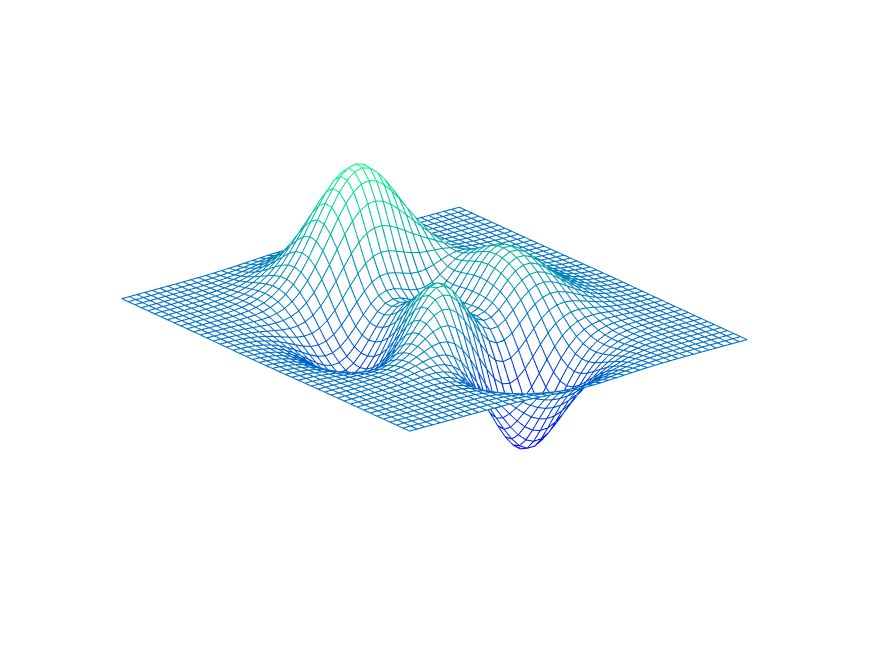
\includegraphics[trim={0cm 0cm 0cm 0cm},clip,height=0.2\textheight,width=1\linewidth,keepaspectratio]{../Figures/Plain/exfigure1} \\
							\end{center}
							\vspace{-0.5cm}
							\caption{Subfigure A} \label{subfig:exsubfigureA}
							\vspace{0.5cm}
						\end{subfigure}
						
						\begin{subfigure}[t]{\linewidth}
							\begin{center}
								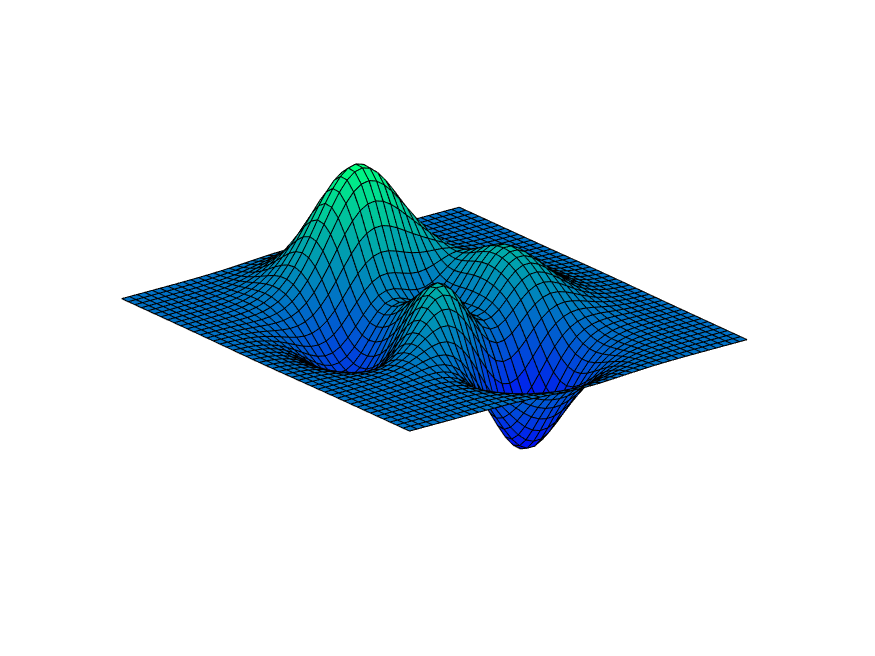
\includegraphics[trim={0cm 0cm 0cm 0cm},clip,height=0.2\textheight,width=1\linewidth,keepaspectratio]{../Figures/Plain/exfigure2} \\
							\end{center}
							\vspace{-0.5cm}
							\caption{Subfigure B} \label{subfig:exsubfigureB}
							\vspace{0.5cm}
						\end{subfigure}
					\fignotes{ Add standalone description. \iftoggle{longnotes}{Long for text.}{Short for slides.} 
						You can reference (dynamic) variables like \lastobs. }
				\end{minipage}
			\end{center}
		\end{figure}
%	}
\end{document}
% trim = {<left> <lower> <right> <upper>}

\end{appendices}}{}	% May need to compile twice (for ToC) and re-run biber (for references)
}{}												% Closes \iftoggle{fulldraft}

\iftoggle{toclinks}{\maketoc}{}		% Table of contents for editing

\end{document}

%---------------------------------------------------------------
% CRediT (Contributor Roles Taxonomy) author statement
%---------------------------------------------------------------
% Author 1: Conceptualization, methodology, data curation, formal analysis. 
% Author 2: Investigation, software, validation, visualization, writing, supervision.

%---------------------------------------------------------------
% Notes
%---------------------------------------------------------------
% To update or remove previously citated references in TexStudio:
% - Tools -> Commands -> Biber
% - Build & View